\section{Processus du second ordre}
\label{sec:stat-second-ordre}


\begin{definition}[Processus du second ordre]
Le processus $X=(X_t)_{t \in T}$ \`a valeurs dans $\Cset^d$ est dit
du second ordre, si $\PE {|X_t|^2} < \infty$ pour tout $t\in T$, o\`u $|x|$
est la norme hermitienne de $x\in \Cset^d$.
\end{definition}
Notons que la \emph{fonction moyenne} d\'efinie sur $T$ par $\mu(t)= \PE{X_t}$
est \`a valeurs dans $\cset^d$ et que la \emph{fonction d'autocovariance}
d\'efinie sur $T\times T$ par
\[
\Gamma(s,t)
   = \cov(X_s,X_t)
   = \PE{(X_s - \mu(s))(X_t-\mu(t))^H}\;.
\]
Elle prend ses valeurs dans l'espace des matrices de dimension $d\times d$. Pour tout $s\in T$, $\Gamma(s,s)$ est une matrice
d'autocovariance. C'est donc une matrice hermitienne positive. Plus
g\'en\'eralement, toute fonction d'autocovariance v\'erifie les propri\'et\'es
suivantes.

\begin{proposition}
 \label{prop:positifcovgene}
 Soit $\Gamma$ la fonction d'autocovariance d'un processus du second ordre
 index\'e par $T$ \`a valeurs dans $\Cset^d$. Elle v\'erifie alors les propri\'et\'es
 suivantes.
\begin{enumerate}
\item
Sym\'etrie hermitienne: pour tout $s,t \in T$,
\begin{equation}\label{eq:gamma_hermitienne}
\Gamma(s,t)= \Gamma(t,s)^H
\end{equation}
\item Type positif \index{Fonction d'autocovariance
\subitem{positivit\'e}}:
pour tout $n\geq1$, pour tout $t_1,\dots,t_n\in T$ et pour tout
$a_1,\cdots,a_n\in\cset^d$,
\begin{equation}
\label{eq:typenonnegatif} \sum_{1 \leq k,m \leq n} a_k^H
 \Gamma(t_k,t_m)a_m \geq 0
\end{equation}
\end{enumerate}
\end{proposition}
\begin{proof}\smartqed
La propri\'et\'e~(\ref{eq:gamma_hermitienne}) est imm\'ediate par d\'efinition de la
covariance.  Pour monntrer~(\ref{eq:typenonnegatif}),
formons la combinaison lin\'eaire $Y= \sum_{k=1}^n a^H_k X_{t_k}$.
$Y$ est une variable al\'eatoire complexe. % Sa variance, qui est
En utilisant les propri\'et\'es de forme hermitienne de la covariance, on obtient
\[
 \Var{Y}= \sum_{1 \leq k,m \leq n} a_k^H
\Gamma(t_k,t_m)a_m
\]
ce qui \'etablit~(\ref{eq:typenonnegatif}).

\end{proof}
Dans le cas scalaire ($d = 1$), on note en g\'en\'eral $\gamma(s,t)$
la covariance, en r\'eservant la notation $\Gamma(s,t)$ au cas des
processus vectoriels ($d > 1$).
%======================================================
%======================================================

\section{Covariance d'un processus stationnaire au second
ordre}

%==================================================
%==================================================
Dor\'enavant, dans ce chapitre, on prend $T=\zset$.  On d\'efinit la stationnarit\'e
au second ordre en ne retenant que les propri\'et\'es du second ordre (moyenne et
covariance) d'un processus stationnaire au sens strict index\'e par $\Zset$.  En
effet, soit $X=(X_{t})_{t \in \Zset}$ un processus stationnaire au sens strict
\`a valeurs dans $\Cset^d$. Supposons de plus qu'il est du second ordre. Alors sa
fonction moyenne est constante puisque la loi marginale l'est, et sa fonction
d'autocovariance $\Gamma$ v\'erifie $\Gamma(s,t)=\Gamma(s-t,0)$ pour tout
$s,t\in\zset$ puisque les lois bi-dimensionnelles sont invariantes par
translation.  Cela donne la d\'efinition suivante.
\begin{definition}[Stationnarit\'e au second ordre]\label{def:statio_sec_ordre}
  Soit $\mu\in\Cset^d$ et $\Gamma:\Zset\to\Cset^{d\times d}$.  Un processus
  $(X_{t})_{t \in \Zset}$ \`a valeurs dans $\Cset^d$ est dit \emph{stationnaire
    au second ordre} (ou \emph{faiblement stationnaire}) de moyenne $\mu$ et de
  \emph{fonction d'auto-covariance} $\Gamma$ si~:
\begin{enumerate}[label=(\alph*)]
\item $X$ est un processus du second ordre, i.e.
$\PE{|X_{t}|^2}<+\infty$,
\item pour tout $t \in \Zset$, $\PE{ X_{t}
}=\mu$,
\item\label{eq:diffgamma} pour tout couple $(s,t) \in \Zset \times \Zset$, $\cov(X_s,X_t)= \Gamma(s-t)$.
\end{enumerate}
\end{definition}

Par convention la fonction d'autocovariance d'un processus stationnaire au
second ordre index\'e par $T$ est d\'efinie sur $T$ au lieu de $T\times T$ pour le
cas g\'en\'eral.

Comme expliqu\'e en pr\'eambule de la d\'efinition, un processus du second ordre
stationnaire au sens strict est stationnaire au second ordre.  L'implication
inverse est vraie pour la classe des processus gaussiens d\'efinies au
paragraphe~\ref{sec:proc-gauss-reels} d'apr\`es la
proposition~\ref{prop:vect_gaussiens}.


On remarque qu'un processus $(X_{t})_{t \in \Zset}$ \`a valeurs dans $\Cset^d$
est stationnaire au second ordre de moyenne $\mu$ et de \emph{fonction
  d'auto-covariance} $\Gamma$ si et seulement si pour tout $\lambda\in\Cset^d$,
le processus $(\lambda^HX_{t})_{t \in \Zset}$ \`a valeurs dans $\Cset$ est
stationnaire au second ordre de moyenne $\lambda^H\mu$ et de \emph{fonction
  d'auto-covariance} $\lambda^H\Gamma\lambda$.  L'\'etude des processus
stationnaires au second ordre peut donc se restreindre au cas $d=1$ sans grande
perte de g\'en\'eralit\'e.





%=========================================================
%=========================================================
%=========================================================
\subsection{Propri\'et\'es}
Les propri\'et\'es de la proposition~\ref{prop:positifcovgene} se d\'eclinent pour un
processus stationnaire au second ordre de la fa\c{c}on suivante.
\begin{proposition}
 \label{prop:stat2}
 La fonction d'autocovariance $\gamma: \Zset \rightarrow \Cset$ d'un processus
 stationnaire au second ordre \`a valeurs complexes v\'erifie les propri\'et\'es
 suivantes qui sont une cons\'equence directe de la proposition
 \ref{prop:positifcovgene}.
\begin{enumerate}
\item Sym\'etrie hermitienne~: \index{Fonction d'autocovariance
\subitem{sym\'etrie hermitienne}} Pour tout $s\in\zset$,
\[
\gamma(-s)= \overline{\gamma(s)}
\]
\item\label{item:type_positif} Type positif~: \index{Fonction
    d'autocovariance \subitem{positivit\'e}} Pour tout entier $n\geq1$ et tout
  vecteur $(a_1, \cdots, a_n)$ de valeurs complexes,
\begin{eqnarray*}
   \sum_{s=1}^{n}\sum_{t=1}^{n}
\overline{a_s} \gamma(s-t) a_t \geq 0
\end{eqnarray*}
\end{enumerate}
\end{proposition}
La matrice de covariance de $n$ valeurs cons\'ecutives $X_1,\dots,X_n$ du
processus poss\`ede de plus une structure particuli\`ere, dite de \emph{Toeplitz},
caract\'eris\'ee par le fait que $(\Gamma_n)_{ij} = \gamma(i-j)$.  On obtient une
matrice de la forme
 \begin{align}
 \Gamma_n \nonumber
      &=\cov([X_1\,\,\dots\,\, X_n]^T) \\
      &=
     \left [
     \begin{matrix}
      \gamma(0)&\gamma(-1)&\cdots&\gamma(1-n)\\
      \gamma(1)&\gamma(0)&\cdots&\gamma(2-n)\\
        \vdots\\
      \gamma(n-1)&\gamma(n-2)&\cdots&\gamma(0)
     \end{matrix}
     \right ]
 \label{eq:matcov}
\end{align}
Lorsque $\gamma(0)$ est non-nul il peut \^{e}tre pratique de normaliser la fonction
d'autocovariance. On obtient la d\'efinition suivante.
\begin{definition}[Fonction d'autocorr\'elation]
  Pour un processus stationnaire au second ordre de variance non nulle, on
  appelle fonction d'autocorr\'elation $\rho$ la fonction d\'efinie sur $s\in\zset$
  par $\rho(s)= \gamma(s)/\gamma(0)$. Il s'agit d'une quantit\'e normalis\'ee dans
  le sens o\`u $\rho(0) = 1$ et $|\rho(s)| \leq 1$ pour tout $s\in\zset$.
\end{definition}
En effet, l'in\'egalit\'e de Cauchy-Schwarz  appliqu\'ee \`a $\gamma$ implique
\[
 |\gamma(s)|
  = \left|\cov(X_{s},X_0)\right| \leq
    \sqrt{\Var{X_{s}}\Var{X_0}} = \gamma(0)
\]
la derni\`ere in\'egalit\'e d\'ecoulant de l'hypoth\`ese de
stationnarit\'e.%  Attention, certaines r\'ef\'erences (livres et
% publications), en g\'en\'eral anciennes, utilisent (incorrectement) le
% terme de ``fonction d'autocorr\'elation'' pour $\gamma(h)$.
% Dans la
% suite de ce document, le terme autocorr\'elation est r\'eserv\'ee \`a la
% quantit\'e normalis\'ee $\rho(h)$.
\begin{example}[Retournement du temps (suite)]
  \label{exe:stat_retourne} Soit $(X_t)_{t\in\zset}$ un processus al\'eatoire
  stationnaire au second ordre \`a valeurs r\'eelles de moyenne $\mu_X$ et de
  fonction d'autocovariance $\gamma_X$. On note, pour tout $t\in\zset$,
  $Y_t=X_{-t}$ le processus {\it retourn\'e}, comme dans
  l'exemple~\ref{exple:time_reversion}. Alors $Y_t$ est un processus
  stationnaire au second ordre de m\^{e}me moyenne et de m\^{e}me fonction
  d'autocovariance que le processus $X_t$. En effet on a~:
 \begin{align*}
  &\PE{Y_t}= \PE{X_{-t}}=\mu_X\\
  &\cov(Y_{t+h},Y_t)=\cov(X_{-t-h},X_{-t})=\gamma_X(-h)=\gamma_X(h)
 \end{align*}
\end{example}
\begin{definition}[Bruit blanc faible]\index{Bruit blanc!faible}
  On appelle bruit blanc faible un processus al\'eatoire stationnaire au second
  ordre \`a valeurs complexes ou r\'eelles, centr\'e, de fonction d'autocovariance
  $\gamma$ d\'efinie par $\gamma(0)= \sigma^2>0$ et $\gamma(s)=0$  pour tout
  $s\neq0$. On le notera $ (X_{t}) \sim  \BB(0,\sigma^2)$.
\end{definition}
\begin{definition}[Bruit blanc fort]\index{Bruit blanc!fort}
On appelle bruit blanc fort une suite de variables
al\'eatoires $(X_{t})$, centr\'ees, ind\'ependantes et identiquement
distribu\'ees (i.i.d.) de variance $\PE{X_{t}^2} = \sigma^2 <
\infty$. On le notera $ (X_{t}) \sim \BBF(0,\sigma^2)$.
\end{definition}
Par d\'efinition un bruit blanc fort est un bruit blanc faible. La
structure de bruit blanc fort est clairement plus contraignante
que celle du  bruit blanc faible. % En g\'en\'eral, il est tout \`a fait
% inutile de faire un telle hypoth\`ese lorsque l'on s'int\'eresse \`a
% des processus  stationnaires au second ordre.
% Il arrivera cependant dans la suite que nous adoptions cette
% hypoth\`ese plus forte afin de simplifier les d\'eveloppements
% math\'ematiques.
Notons que, de m\^{e}me que la stationnarit\'e stricte  d'un processus
gaussien d\'ecoule de la stationnarit\'e
faible, un bruit blanc faible gaussien est un bruit blanc fort.

\begin{example}[Processus MA(1)]
 \label{exe:MA1covth}
Soit $(X_{t})$ le processus stationnaire au second ordre
d\'efini par~:
\begin{equation}
\label{eq:recurrenceMA1}
 X_{t}= Z_{t} + \theta Z_{t-1} \; ,
\end{equation} o\`u $(Z_{t}) \sim \BB(0,\sigma^2)$ r\'eel et $\theta \in
\Rset$. On v\'erifie ais\'ement que $\PE{X_{t}}= 0$ et que sa fonction
d'autocovariance est d\'efinie par
\begin{equation}
  \label{eq:ma1-cov}
\gamma(s)=
\begin{cases}
  \sigma^2(1+\theta^2) & \text{si $s=0$,} \\
  \sigma^2 \theta & \text{si $s=\pm 1$,} \\
  0 & \text{sinon.}
\end{cases}
\end{equation}
Le processus $(X_{t})$ est donc bien stationnaire au second ordre.
Un tel processus est appel\'e \emph{processus \`a moyenne ajust\'ee d'ordre 1}.
Cette propri\'et\'e se g\'en\'eralise, sans difficult\'e, \`a un processus
MA($q$). Nous reviendrons plus en d\'etail, paragraphe
\ref{s:procARMA}, sur la d\'efinition et les propri\'et\'es de ces
processus.
\end{example}
\begin{example}[Processus harmonique r\'eel]
  \label{ex:processusharmonique} Soient $(A_k)_{1 \leq k \leq N}$ $N$
  v.a. r\'eelles de variance finie. On note $\sigma_k^2=\Var{A_k}$. Soient
  $(\Phi_k)_{1 \leq k \leq N}$, $N$ variables al\'eatoires ind\'ependantes et
  identiquement distribu\'ees (i.i.d), de loi uniforme sur $[-\pi,\pi]$, et
  ind\'ependantes de $(A_k)_{1 \leq k \leq N}$. On d\'efinit~:
\begin{equation}
   X_{t} = \sum_{k=1}^N A_k \cos(\lambda_k t + \Phi_k ) \;,
\end{equation}
o\`u $(\lambda_k)_{1 \leq k \leq N}\in [- \pi,\pi]$ sont $N$ pulsations. Le
processus $(X_{t})$ est appel\'e processus harmonique. On v\'erifie ais\'ement que
$\PE {X_{t}}= 0$ et que, pour tout $s,t\in\zset$,
\[
\PE{X_{s}X_{t}} = \frac{1}{2}
     \sum_{k=1}^N \sigma_k^2 \cos ( \lambda_k (s-t) ) \;.
\]
Le processus harmonique est donc stationnaire au second ordre.
\end{example}
\begin{example}[Marche al\'eatoire]
\label{ex:marche_aleatoire} Soit $(S_{t})$ le processus d\'efini sur
$t \in \Nset$ par $S_{t}= X_{0} + X_{1} + \cdots + X_{t}$, o\`u
$(X_{t})$ est un bruit blanc fort r\'eel. Un tel processus est appel\'e
\emph{une marche al\'eatoire}. On en d\'eduit que $\PE{S_{t}}= 0$,
$\PE{S_t^2}=t\sigma^2$ et, pour $s\leq t\in\nset$, on a~:
\[
\PE{S_sS_t} = \PE{ (S_{s} + X_{s+1} + \cdots + X_{t})S_{s}}
    = s \; \sigma^2
\]
Le processus $(S_{t})$ n'est donc pas stationnaire au second
ordre.
\end{example}
\begin{example}
 \label{exe:testposivite1}
Nous allons montrer que la fonction $\chi$ d\'efinie sur $\zset$, par
\begin{equation}
  \label{eq:covma1chi}
 \chi(s)=
 \begin{cases}
  1 & \text{si $s=0$,} \\
  \rho & \text{si $s=\pm 1$,} \\
  0 & \text{sinon.}
 \end{cases}
\end{equation}
est la fonction d'autocovariance d'un processus stationnaire au
second ordre r\'eel si et seulement si $\rho \in [-1/2,1/2]$. Nous avons d\'ej\`a
montr\'e exemple \ref{exe:MA1covth} que la fonction d'autocovariance
$\gamma$ d'un processus MA(1) est donn\'ee par~(\ref{eq:ma1-cov}).
La fonction $\chi$ est donc la fonction d'autocovariance d'un
processus MA(1) si et seulement si $\sigma^2(1+\theta^2)= 1$ et
$\sigma^2 \theta = \rho$. Lorsque $|\rho| \leq 1/2$, ce
syst\`eme d'\'equations admet comme solution~:
\[
 \theta = (2 \rho)^{-1}( 1 \pm \sqrt{1 - 4 \rho^2})
 \quad\mbox{et}\quad
 \sigma^2= (1+ \theta^2)^{-1}\;.
\]
Lorsque $|\rho| > 1/2$, ce syst\`eme d'\'equations n'admet pas de solution r\'eelles
et la fonction $\chi$ n'est donc pas la fonction d'autocovariance d'un
processus MA(1). Plus g\'en\'eralement, si $|\rho|>1/2$, alors $\chi$ n'est en
fait pas de type positif et n'est donc pas une fonction de covariance,
voir Proposition~\ref{prop:stat2}.
\end{example}

\subsection{Interpr\'etation de la fonction d'autocovariance}
\label{sec:interp_cov} Dans les exemples pr\'ec\'edents, nous avons
\'et\'e amen\'es \`a \'evaluer la fonction d'autocovariance de processus pour
quelques exemples simples de s\'eries temporelles. Dans la plupart
des probl\`emes d'int\'er\^{e}t pratique, nous ne
partons pas de mod\`eles de s\'erie temporelle d\'efinis \emph{a
priori}, mais d'\emph{observations}, $\{ x_1, \dots, x_n\}$
associ\'ees \`a une \emph{r\'ealisation} du processus. Afin de
comprendre la structure de d\'ependance entre les diff\'erentes
observations, nous serons amen\'es \`a
\emph{estimer} la loi du processus, ou du moins des caract\'eristiques de ces lois.
Pour un processus stationnaire au second ordre, nous pourrons, \`a titre d'exemple, estimer
sa moyenne par la \emph{moyenne empirique}~:
\[
 \hat\mu_n = n^{-1} \sum_{k=1}^n x_k
\]
et les fonctions d'autocovariance et d'autocorr\'elation par les
fonctions d'autocorr\'elation et d'autocovariance \emph{empiriques}
\[
 \hat{\gamma}(h) = n^{-1} \sum_{k=1}^{n - |h|} (x_k - \hat\mu_n)(x_{k+|h|} - \hat\mu_n)
 \quad\mbox{et}\quad
 \hat{\rho}(h) = \hat{\gamma}(h) / \hat{\gamma}(0)\;.
\]
Lorsqu'il est \emph{a priori} raisonnable de penser que la s\'erie
consid\'er\'ee est stationnaire au second ordre, la moyenne empirique,
la fonction d'autocovariance empirique et la fonction
d'autocorr\'elation empirique sont des estimateurs consistants de la fonction d'autocovariance
et de la fonction d'autocorr\'elation.

L'analyse de la fonction d'autocovariance empirique est un \'el\'ement
permettant de guider le choix d'un mod\`ele appropri\'e pour les
observations. Par exemple, le fait que la fonction
d'autocovariance empirique soit \emph{proche} de z\'ero pour tout
$h \ne 0$ (proximit\'e qu'il faudra d\'efinir dans un sens statistique
pr\'ecis) indique par exemple qu'un bruit blanc est un mod\`ele
ad\'equat pour les donn\'ees. La figure \ref{fig:xcorrhr} repr\'esente
les $100$ premi\`eres valeurs de la fonction d'autocorr\'elation
empirique de la s\'erie des battements cardiaques repr\'esent\'ee figure
\ref{fig:figcard1}. On observe que cette s\'erie est
\emph{positivement corr\'el\'ee} c'est-\`a-dire que les fonctions
coefficients d'autocorr\'elation sont positifs et significativement
non nuls. Nous avons, \`a titre de comparaison, repr\'esent\'e aussi la
fonction d'autocorr\'elation empirique d'une trajectoire de m\^{e}me
longueur d'un bruit blanc gaussien.
 %=========== FIGURE =====================
\begin{figure}
  \centering
  % Requires \usepackage{graphicx}
  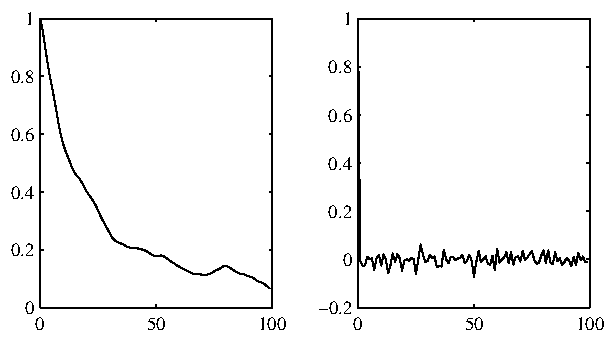
\includegraphics[width=0.6\textwidth]{Figures/corrHR11839}\\
  \caption{Courbe de gauche~: fonction d'autocorr\'elation empirique de la s\'erie
 des battements cardiaques (figure \ref{fig:figcard1}). Courbe de droite~:
 fonction d'autocorr\'elation
 empirique d'une trajectoire de m\^{e}me longueur d'un bruit blanc
 gaussien.}\label{fig:xcorrhr}
\end{figure}
 La figure~\ref{fig:xcov} montre que le fait que $\hat{\rho}(1)
 = 0.966$ pour la s\'erie des battements cardiaques se traduit par une forte
 pr\'edictabilit\'e de $X_{t+1}$ en fonction de $X_t$ (les couples de points
 successifs s'alignent quasiment sur une droite). Nous montrerons au
 chapitre~\ref{chap:Prediction}, que dans un tel contexte,
 $\PE{(X_{t+1}-\mu)-\rho(1)(X_t-\mu)} = (1-\rho^2) \cov(X_t)$, c'est-\`a-dire,
 compte tenu de la valeur estim\'ee pour $\rho(1)$, que la variance de ``l'erreur
 de pr\'ediction'' $X_{t+1}-[\mu+\rho(1)(X_t-\mu)]$ est 15 fois plus faible que
 celle du signal original.
 %=========== FIGURE =====================
\begin{figure}
  \centering
  % Requires \usepackage{graphicx}
  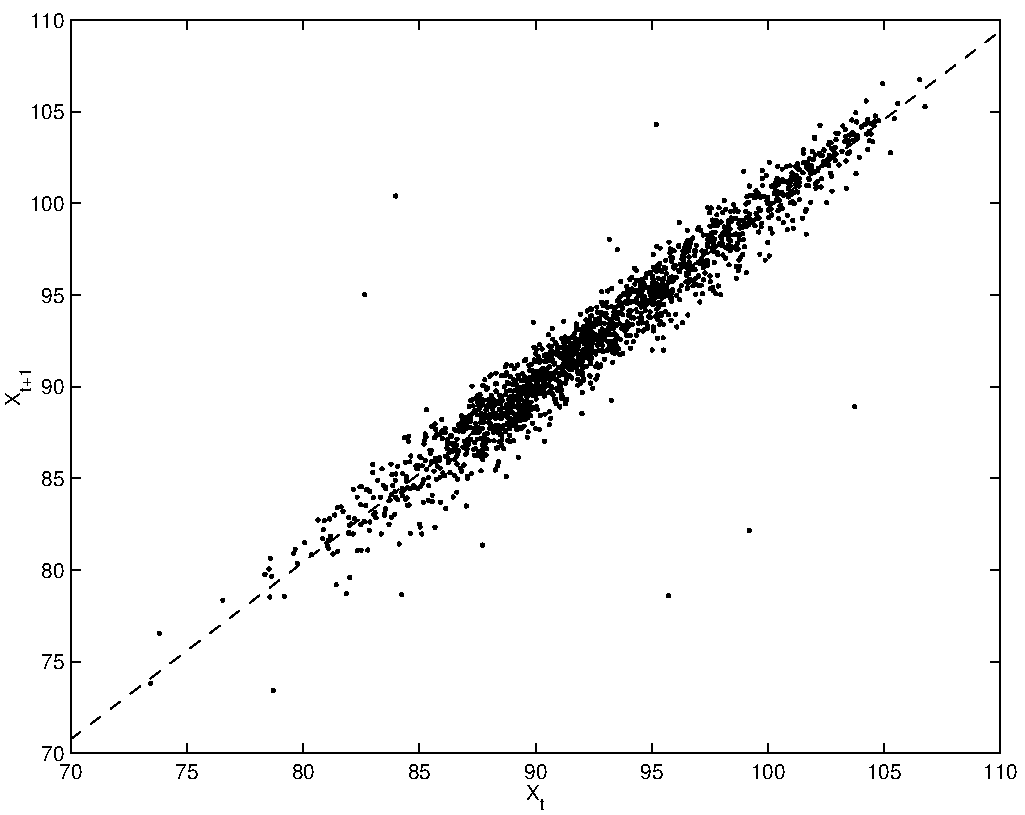
\includegraphics[width=0.6\textwidth]{Figures/cov_hr11839}\\
  \caption{$X_{t+1}$ en fonction de $X_t$ pour la s\'erie
 des battements cardiaques de la figure~\ref{fig:figcard1}. Les tirets
 repr\'esentent la meilleure droite de r\'egression lin\'eaire de $X_{t+1}$ sur $X_t$.}
 \label{fig:xcov}
\end{figure}

\begin{figure}
  \centering
  % Requires \usepackage{graphicx}
  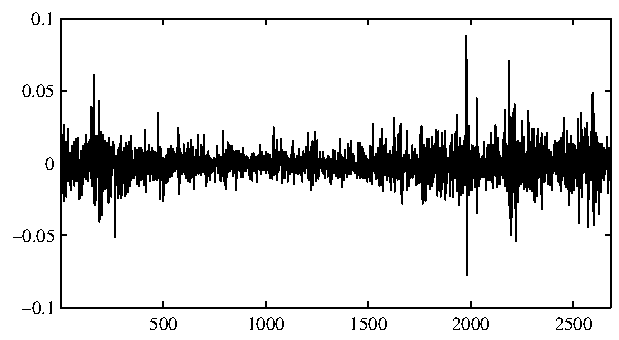
\includegraphics[width=0.6\textwidth]{Figures/logretourSP}\\
  \caption{Log-Retours de la s\'erie S\&P 500}\label{fig:sp-logretour}
\end{figure}
 L'indice S\&P$500$ trac\'e (fig.~\ref{fig:SP}) pr\'esente un cas de figure plus
 difficile, d'une part parce que la s\'erie n'est clairement pas
 stationnaire~; d'autre part, parce que selon le choix de la transformation des
 donn\'ees consid\'er\'ees, la s\'erie transform\'ee pr\'esente ou non des effets de
 corr\'elation. On d\'efinit tout d'abord les \emph{log-retours} de l'indice
 S\&P$500$ comme les diff\'erences des logarithmes de l'indice \`a deux dates
 successives~:
\[
 X_{t} = \log( S_{t}) - \log(S_{t-1})
      = \log \left( 1 + \frac{S_{t}-S_{t-1}}{S_{t-1}} \right)
\]
La s\'erie des log-retours de la s\'erie S\&P 500 est repr\'esent\'ee dans la
figure \ref{fig:sp-logretour}.
 %=========== FIGURE =====================

\begin{figure}
  \centering
  % Requires \usepackage{graphicx}
  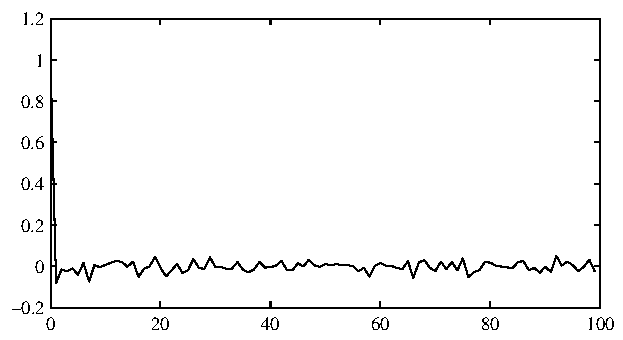
\includegraphics[width=0.6\textwidth]{Figures/corrsplogretour}\\
  \caption{Fonction d'autocorr\'elation empirique de la s\'erie des log-retours
 de l'indice S\&P 500.}\label{fig:sp-xcorr}
\end{figure}
  Les coefficients d'autocorr\'elation
empiriques de la s\'erie des log-retours sont repr\'esent\'es dans la figure
\ref{fig:sp-xcorr}. On remarque qu'ils sont approximativement nuls
pour $h \ne 0$ ce qui sugg\`ere de mod\'eliser la s\'erie des
log-retours par un bruit blanc faible.
  %=========== FIGURE =====================
\begin{figure}
  \centering
  % Requires \usepackage{graphicx}
  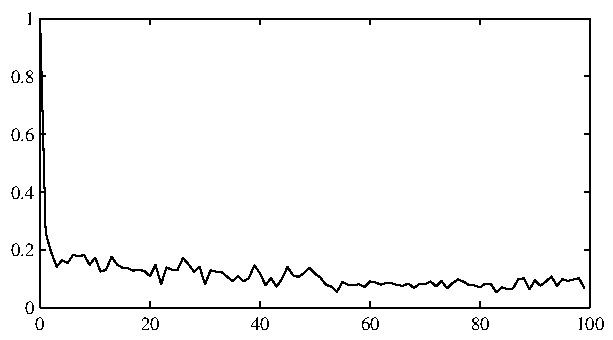
\includegraphics[width=0.6\textwidth]{Figures/corrabssplogretour}\\
  \caption{Fonction d'autocorr\'elation empirique de la s\'erie des valeurs absolues des
 log-retours de l'indice S\&P 500.}\label{fig:sp-abs-xcorr}
\end{figure}
Il est int\'eressant d'\'etudier aussi la s\'erie des log-retours
absolus, $A(t) = |X_{t}|$. On peut, de la m\^{e}me fa\c{c}on,
d\'eterminer la suite des coefficients d'autocorr\'elation empirique
de cette s\'erie, qui est repr\'esent\'ee dans la figure
\ref{fig:sp-abs-xcorr}. On voit, qu'\`a l'inverse de la s\'erie des
log-retours, la s\'erie des valeurs absolues des log-retours est
positivement corr\'el\'ee, les valeurs d'autocorr\'elation \'etant
significativement non nulles pour $|h| \leq 100$. On en d\'eduit, en
particulier, que la suite des log-retours peut \^{e}tre mod\'elis\'ee
comme un bruit blanc, mais pas un bruit blanc fort\,: en effet,
pour un bruit blanc fort $X_{t}$, nous avons, pour toute fonction
$f$ telle que $\PE{f(X_{t})^2} = \sigma_f^2 < \infty$,
$\cov(f(X_{t+h}),f(X_{t}))= 0$ pour $h\neq 0$ (les variables
$f(X_{t+h})$ et $f(X_{t})$ \'etant ind\'ependantes, elles sont a
fortiori non corr\'el\'ees).
%==================================================
%==================================================
\section{Mesure spectrale d'un processus stationnaire}
%==================================================
Dans toute la suite, $\tore$ d\'esigne le tore $\ocint{-\pi,\pi}$ et
$\btore$ la tribu bor\'elienne associ\'ee. Le th\'eor\`eme
d'Herglotz ci dessous \'etablit l'\'equivalence entre la fonction
d'autocovariance et une mesure finie d\'efinie sur
$(\tore,\btore)$. Cette mesure, appel\'ee \emph{mesure
  spectrale du processus}, joue un r\^ole analogue \`a celui de la transformation
de Fourier pour les fonctions de carr\'e int\'egrable.
%================== HERGLOTZ =======================
\begin{theorem}[Herglotz]
\label{theo:herglotz}
 Une suite $(\gamma(h))_{h \in
\Zset}$ est de type positif si et seulement si il existe une unique
mesure positive $\nu$ sur $(\tore,\btore)$ telle que~:
\begin{eqnarray}
\label{eq:herglotz}
 \gamma(h) = \int_{\tore} \rme^{\rmi h\lambda} \nu(\rmd\lambda),\; \forall h\in\Zset\;.
\end{eqnarray}
%  Si la suite $(\gamma(h))$ est de carr\'e sommable
% (\textit{i.e.} $\sum_{h\in \zset} \gamma^2(h)<\infty$),
% la mesure $\nu$ poss\`ede une densit\'e $f$ (\textbf{fonction
% positive}) par rapport \`a la mesure de Lebesgue sur
% $(\tore,\btore)$ et s'\'ecrit donc
% $$
% \gamma(h) = \int_{\tore} \rme^{\rmi h\lambda} f(\lambda)\rmd\lambda\; ,
% $$
% o\`u $f$ est donn\'ee par la s\'erie de Fourier (convergente dans $\ltwo(\tore,\lleb)$ \footnote{voir Th\'eor\`eme~\ref{theo:convergence-series-fourier}})
% \[
%  f(\lambda)= \frac{1}{2\pi} \sum_{k \in \Zset} \gamma(k) \rme^{-\rmi k \lambda}\; .
% \]
\end{theorem}
Lorsque $\gamma$ est la fonction d'autocovariance d'un processus
stationnaire au second ordre, on sait d'apr\`es la proposition
\ref{prop:stat2} que $\{\gamma(h)\}_{h \in
\Zset}$ est de type positif. Les hypoth\`eses du th\'eor\`eme de Herglotz
sont donc v\'erifi\'ees et dans ce cas
la mesure $\nu$ est appel\'ee la
\emph{mesure spectrale} du processus.
Si la mesure $\nu$ poss\`ede une densit\'e $f$  par rapport \`a la mesure de Lebesgue sur
 $(\tore,\btore)$ alors  $f$  est
appel\'ee la \emph{densit\'e spectrale de puissance}
du processus.\index{Densit\'e spectrale}

\begin{proof}
 Si $\gamma(n)$ a la
repr\'esentation~(\ref{eq:herglotz}), montrons que $\gamma(n)$
est de type positif. En effet, pour tout $n$ et toute suite
$\{a_k\in\mathbb{C}\}_{1\leq k\leq n}$,
$$
 \sum_{k,m} a_k\overline{a_m} \gamma(k-m)=
 \int_{\tore} \sum_{k,m} a_k\overline{a_m} \rme^{\rmi k \lambda}\rme^{-im \lambda} \nu(\rmd\lambda)=
 \int_{\tore}\left| \sum_{k} a_k \rme^{\rmi k \lambda}\right|^2 \nu(\rmd\lambda)\geq 0\;.
 $$
 R\'eciproquement, supposons que $\gamma(n)$ soit une suite de type
 positif et consid\'erons la suite de fonctions index\'ee par $n$~:
\[
 f_n(\lambda)
 = \frac{1}{2\pi n} \sum_{k=1}^n \sum_{m=1}^n \gamma(k-m) \rme^{-\rmi k \lambda} \rme^{\rmi m\lambda}
 = \frac{1}{2\pi}\sum_{k=-(n-1)}^{n-1} \left( 1 - \frac{|k|}{n} \right)
                    \gamma(k) \rme^{-\rmi k \lambda}\; .
% = \frac{1}{2\pi}\sum_{k=-\infty}^{\infty}\gamma_n(k)\rme^{-\rmi k \lambda}
\]
$\gamma$ \'etant de type positif, $f_n(\lambda)\geq 0$, pour tout $\lambda\in \tore.$
Notons
$\nu_n$ la mesure (positive) de densit\'e $f_n$ par rapport \`a la mesure de
Lebesgue sur $\tore$. On a alors
\begin{multline}\label{eq:herglotz_1}
\int_{\tore}\rme^{\rmi h \lambda}\nu_n(\rmd\lambda)
=\int_{\tore}\rme^{\rmi h \lambda}f_n(\lambda)\rmd\lambda
=\frac{1}{2\pi}\sum_{k=-(n-1)}^{n-1} \left( 1 - \frac{|k|}{n} \right)
                    \gamma(k) \int_{\tore}\rme^{\rmi (h-k)
                      \lambda}\rmd\lambda\\
=
\left\lbrace
\begin{array}{cc}
\left(1-\frac{|h|}{n}\right)\gamma(h),&\textrm{ si }|h|<n\; ,\\
0,&\textrm{ sinon}\; .
\end{array}
\right.
\end{multline}
% \emnote{Attention \`a ce genre de citations avec des noms.. donc il faut mettre
%   une r\'ef\'erence explicite, dans un ouvrage si possible r\'ecent et diffus\'e, avec
%   des noms. Je ne trouve pas idiot de donner un \'enonc\'e pr\'ecis du th\'eor\`eme. Il
%   manque \`a mon sens dans l'\'enonc\'e et dans la preuve, l'unicit\'e de la limite. Il
%   me semble que le th\'eor\`eme de Prohorov est en g\'en\'eral formul\'e pour des mesures
%   de probabilit\'es, donc des mesures dont la masse totale est constante... du
%   coup, on donne ce th\'eor\`eme dans notre chapitre}
Quitte \`a renormaliser $\nu_n$ pour en faire une mesure de probabilit\'e,
le th\'eor\`eme de Prohorov implique qu'il existe une mesure positive $\nu$ et une sous-suite $\nu_{n_k}$ de
$\nu_n$ telle que
$$
\int_{\tore}\rme^{\rmi h\lambda}\nu_{n_k}(\rmd\lambda)
\longrightarrow \int_{\tore}\rme^{\rmi h\lambda}\nu(\rmd\lambda),
\textrm{ lorsque }k\to\infty\;.
$$
En rempla\c{c}ant $n$ par $n_k$ dans \eqref{eq:herglotz_1} et en faisant
tendre $k$ vers l'infini, on a
$$
\gamma(h)=\int_{\tore}\rme^{\rmi h \lambda}\nu(\rmd\lambda),\; \forall h\in\Zset\;.
$$
Montrons \`a pr\'esent que $\nu$ est unique. En effet, s'il existait une autre mesure
$\mu$ telle que pour tout $h\in\Zset$ : $\int_{\tore}\rme^{\rmi h
  \lambda}\nu(\rmd\lambda)=\int_{\tore}\rme^{\rmi h
  \lambda}\mu(\rmd\lambda)$
alors d'apr\`es le lemme \ref{lem:approxLinfini-convol-noyau},
$\int_{\tore}
g(\lambda)\nu(\rmd\lambda)=\int_{\tore}g(\lambda)\mu(\rmd\lambda)$
pour toute fonction continue $g$ telle que $g(\pi)=g(-\pi)$.
On en d\'eduit donc que $\nu=\mu$.

\end{proof}

\begin{corollary}[Corollaire du th\'eor\`eme d'Herglotz]
\label{prop:testpositif}
 Une suite $(\gamma(h))_{h \in \Zset}$ \`a valeurs complexes telle que
 $\sum_{h\in \zset} |\gamma(h)|^2<\infty$ est de type
positif si et seulement si la fonction d\'efinie par
$$
 f(\lambda)=\frac{1}{2\pi}\sum_{h\in\mathbb{Z}} \gamma(h)\rme^{-\rmi h \lambda}
$$
est positive pour tout $\lambda \in \mathbb{T}$.
\end{corollary}

\begin{proof}\smartqed
D'apr\`es le th\'eor\`eme de Herglotz (Th\'eor\`eme \ref{theo:herglotz}),
$(\gamma(h))_{h \in \Zset}$ est de type
positif si et seulement si il existe une mesure positive
 $\nu$ sur $(\tore,\btore)$ telle que~:
\begin{eqnarray*}
 \gamma(h) = \int_{\tore} \rme^{\rmi h\lambda} \nu(\rmd\lambda)\; .
\end{eqnarray*}
D'apr\`es le th\'eor\`eme~\ref{theo:convergence-series-fourier} et le
corollaire \ref{cor:completude-base-l2}, comme $\sum_{h\in \zset} |\gamma(h)|^2<\infty$, on peut consid\'erer
la s\'erie de Fourier associ\'ee convergente dans
$\ltwo(\tore,\lleb)$ :
$(2\pi)^{-1} \sum_{k \in \Zset} \gamma(k) \rme^{-\rmi k
  \lambda}\eqdef f(\lambda)$.
Ainsi, $\gamma(h) = \int_{\tore} \rme^{\rmi h\lambda} f(\lambda)\rmd\lambda$
et donc la positivit\'e de $\nu$ revient \`a la positivit\'e de $f$, ce qui
conclut la preuve.


% Supposons tout d'abord que $\gamma$ est absolument sommable et
% montrons que si $f(\lambda)$ d\'efinie dans la proposition est positive
% sur $\tore$ alors $\{\gamma(h)\}$ est de type positif. D'apr\`es
% \eqref{eq:herglotz_2},
% $\gamma(h)=\int_\tore \rme^{\rmi h\lambda}f(\lambda)\rmd\lambda$.
% Comme $f(\lambda)\geq 0$, $f(\lambda)\rmd\lambda$ d\'efinit bien une
% mesure positive sur $\tore$ et donc d'apr\`es le th\'eor\`eme de
% Herglotz, $\{\gamma(h)\}$ est de type positif.

% Supposons \`a pr\'esent que $\{\gamma(h)\}$ est de type positif et
% absolument sommable et montrons que $f(\lambda)$ d\'efinie dans la proposition est positive
% sur $\tore$. On a
% \emnote{pourquoi on refait la preuve ? si $\gamma(h)$ est de type positif et absolument sommable, Herglotz montre que sa mesure
% spectrale a une densit\'e par rapport \`a la mesure de Lebesgue, non ?}
% \begin{multline*}
% 0\leq f_n(\lambda)=\frac{1}{2\pi n}\sum_{1\leq r,s\leq n}
% \rme^{-\rmi r\lambda}\gamma(r-s)\rme^{\rmi s\lambda}\\
% =\frac{1}{ 2\pi}\sum_{|m|<n}\left(1-\frac{|m|}{n}\right)\rme^{-\rmi m\lambda}\gamma(m)
% \to \frac{1}{2\pi}\sum_{m\in\mathbb{Z}}\gamma(m)\rme^{-\rmi m\lambda}=f(\lambda),\textrm{ lorsque }n\to\infty\;,
% \end{multline*}
% d'apr\`es le th\'eor\`eme de convergence domin\'ee que l'on peut appliquer
% puisque $\sum_{h}|\gamma(h)|<\infty$.
% Ainsi $f(\lambda)\geq 0$ comme limite de fonctions positives.

\end{proof}
\begin{example}
En reprenant l'exemple~\ref{exe:testposivite1}, on v\'erifie
imm\'ediatement que $(\chi(h))$ est de module sommable et que\,:
$$
 f(\lambda)=\frac{1}{2\pi}\sum_h \chi(h)\rme^{-\rmi h \lambda}
     =\frac{1}{2\pi}(1+2\rho\cos( \lambda))
     $$
     et donc que la s\'equence est une fonction d'autocovariance uniquement
     lorsque $|\rho|\leq 1/2$.
\end{example}
\begin{example}[Densit\'e spectrale de puissance du bruit blanc]
  La fonction d'autocovariance d'un bruit blanc est donn\'ee par $\gamma(h)=
  \sigma^2 \delta(h)$, d'o\`u l'expression de la densit\'e spectrale correspondante
\[
 f(\lambda) = \frac{\sigma^2}{2\pi}
\]
La densit\'e spectrale d'un bruit blanc est donc constante. Cette
propri\'et\'e est \`a l'origine de la terminologie ``bruit blanc'' qui
provient de l'analogie avec le spectre de la lumi\`ere blanche
constant dans toute la bande de fr\'equences visibles.
\end{example}
\begin{example}[Densit\'e spectrale de puissance du processus MA(1)]
  \label{ex:MA1dsp}
  Le processus MA(1) introduit dans l'exemple~\ref{exe:MA1covth} poss\`ede une
  s\'equence d'autocovariance donn\'ee par $\gamma(0) = \sigma^2(1+\theta^2)$,
  $\gamma(1) = \gamma(-1) = \sigma^2 \theta$ et $\gamma(h) = 0$ sinon (cf.
  exemple~\ref{exe:MA1covth}). D'o\`u l'expression de sa densit\'e spectrale~:
\[
 f(\lambda)= \frac{\sigma^2}{2 \pi} (2 \theta \cos(\lambda) + (1+ \theta^2))
     = \frac{\sigma^2}{2 \pi} \left |1+ \theta \rme^{-\rmi\lambda}\right |^2
\]
La densit\'e spectrale d'un tel processus est repr\'esent\'ee figure
\ref{fig:dspthMA1} pour $\theta = -0.9$ et $\sigma^2=1$ avec une
\'echelle logarithmique (dB).
\end{example}
 %================ FIGURE
\begin{figure}
  \centering
  % Requires \usepackage{graphicx}
  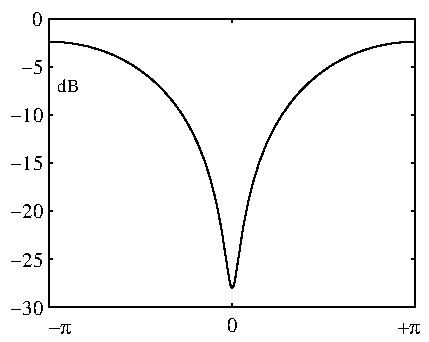
\includegraphics[width=0.6\textwidth]{Figures/dspthMA1}\\
  \caption{Densit\'e spectrale (en dB) d'un processus MA-1, d\'efini par l'\'equation
~(\ref{eq:recurrenceMA1}) pour $\sigma=1$ et $\theta=-0.9$.}\label{fig:dspthMA1}
\end{figure}

\begin{example}[Mesure spectrale du processus harmonique]
La fonction d'autocovariance du processus harmonique $X_{t} =
\sum_{k=1}^N A_k \cos(\lambda_k t + \Phi_k )$ (voir exemple
\ref{ex:processusharmonique}) est donn\'ee par~:
\begin{equation}
 \label{eq:cov_harm}
 \gamma(h) = \frac{1}{2} \sum_{k=1}^N \sigma_k^2
  \cos ( \lambda_k h)
\end{equation}
o\`u $\sigma_k^2=\PE{A_k^2}$. Cette suite de coefficients
d'autocovariance n'est pas sommable et la mesure spectrale n'admet
pas de densit\'e. En notant cependant que~:
\[
 \cos(\lambda_k h)
 = \frac{1}{2} \int_{- \pi}^{\pi} \rme^{\rmi  h \lambda}
 (\delta_{\lambda_k}(\rmd\lambda) + \delta_{-\lambda_k}(\rmd\lambda))
\]
o\`u $\delta_{x_0}(\rmd\lambda)$ d\'esigne la mesure de Dirac au
point $x_0$ (cette mesure associe la valeur $1$ \`a tout bor\'elien de
$[-\pi,\pi]$ contenant $x_0$ et la valeur $0$ sinon), la mesure
spectrale du processus harmonique peut s'\'ecrire~:
\[
 \nu(\rmd\lambda)=
    \frac{1}{4} \sum_{k=1}^N \sigma_k^2 \delta_{\lambda_k}(\rmd\lambda)
    +
    \frac{1}{4} \sum_{k=1}^N \sigma_k^2 \delta_{-\lambda_k}(\rmd\lambda)
\]
Elle appara\^{i}t donc comme une somme de mesures de Dirac, dont
les masses $\sigma_k^2$ sont localis\'ees aux pulsations des
diff\'erentes composantes harmoniques.
\end{example}
Contrairement aux autres exemples
\'etudi\'es, le processus harmonique poss\`ede une fonction d'autocovariance, donn\'ee
par~\ref{eq:cov_harm}, non absolument sommable ($\gamma(h)$ ne
tend pas m\^{e}me vers 0 pour les grandes valeurs de $h$). Par suite, il admet une mesure spectrale mais pas une densit\'e
spectrale. La propri\'et\'e suivante, \`a d\'emontrer \`a titre d'exercice,
implique que le processus harmonique est en fait enti\`erement
pr\'edictible \`a partir de quelques-unes de ses valeurs pass\'ees.
\begin{proposition}
  S'il existe un rang $n$ pour lequel la matrice de covariance $\Gamma_n$
  d\'efinie en (\ref{eq:matcov}) est non inversible, le processus correspondant
  $X_t$ est pr\'edictible dans le sens o\`u il existe une combinaison lin\'eaire
  $a_1, \dots a_{l}$ avec $l \leq n-1$ telle que $X_t = \sum_{k=1}^l a_k
  X_{t-k}$, l'\'egalit\'e ayant lieu presque s\^urement.
\end{proposition}
L'expression de la fonction d'autocovariance, obtenue
en~(\ref{eq:cov_harm}) pour le processus harmonique, montre que
les matrices de covariances associ\'ees s'\'ecrivent comme la somme de
$2 N$ matrices complexes de rang 1. Par cons\'equent, les matrices
$\Gamma_n$ ne sont pas inversibles d\`es que $n > 2N$, ce qui
implique que le processus harmonique est pr\'edictible d\`es lors
que l'on en a observ\'e $2N$ valeurs. Ce r\'esultat est sans surprise
compte tenu du fait que les trajectoires de ce processus sont des
sommes de sinuso\"{i}des de fr\'equences $\lambda_1,\dots,
\lambda_N$ dont seules les amplitudes et les phases sont
al\'eatoires. La propri\'et\'e suivante donne une condition suffisante
simple pour \'eviter ce type de comportements ``extr\^{e}mes''.
Cette propri\'et\'e implique en particulier que, pour une fonction
d'autocovariance absolument sommable (tous les exemples vus
ci-dessus en dehors du processus harmoniques), les valeurs futures
du processus correspondant ne sont pas pr\'edictibles sans erreur \`a
partir d'un ensemble fini de valeurs pass\'ees du processus. Nous
reviendrons en d\'etail sur ces probl\`emes de pr\'ediction au
chapitre~\ref{chap:Prediction}.
\begin{proposition}
 \label{prop:Gammanrangplein}
Soit $\gamma(h)$ la fonction d'autocovariance d'un processus
stationnaire au second ordre. On suppose que $\gamma(0)>0$ et que
$\gamma(h)\rightarrow 0$ quand $h\rightarrow \infty$. Alors, quel
que soit $n$, la matrice de covariance d\'efinie
en~(\ref{eq:matcov}) est de rang plein et donc inversible.
\end{proposition}
\begin{proof}\smartqed
% autre demo pp 167 du brockwell
 Supposons qu'il existe une suite de valeurs complexes $(a_1,\dots,a_n)$
non toutes nulles, telle que $\sum_{k=1}^n\sum_{m=1}^n a_k \overline{a_m}
\gamma(k-m)=0$. En notant $\nu_X$ la mesure spectrale de $X_t$, on
peut \'ecrire~:
\begin{eqnarray*}
  0
    =\sum_{k=1}^n\sum_{m=1}^n a_k \overline{a_m}
\int_{\tore} \rme^{\rmi(k-m)\lambda}\nu_X(\rmd\lambda)
    =\int_{\tore} \left| \sum_{k=1}^n a_k \rme^{\rmi k \lambda}\right|^2 \nu_X(\rmd\lambda)
\end{eqnarray*}
Ce qui implique que $| \sum_{k=1}^n a_k \rme^{\rmi k \lambda}|^2=0$ $\nu_X$ presque partout, c'est \`a dire que $$
\nu_X(\{\lambda
: \left| \sum_{k=1}^n a_k \rme^{\rmi k \lambda}\right|^2\neq 0\})=\nu_X(\tore-Z)=0
$$
o\`u
$Z=\{\lambda_1,\dots,\lambda_M\,: \sum_{k=1}^n a_k \rme^{\rmi k \lambda_m}
= 0\}$ d\'esigne l'ensemble \emph{fini} ($M<n$) des racines $x\in \tore$
du polyn\^ome trigonom\'etrique $\sum_{k=1}^n a_k \rme^{\rmi k \lambda}$. Par
cons\'equent, les seuls \'el\'ements de $\btore$, qui peuvent \^{e}tre
de mesure non nulle pour $\nu_X$, sont les singletons
$\{\lambda_m\}$. Ce qui implique que $\nu_X=\sum_{m=1}^M a_m
\delta_{\lambda_m}$ (o\`u $a_m\geq 0$ ne peuvent \^{e}tre tous
nuls si $\gamma(0)\neq 0$). Mais, dans ce cas,
$\gamma(h)=\sum_{m=1}^M a_m \rme^{\rmi h\lambda_m}$, ce qui contredit
l'hypoth\`ese que $\gamma(h)$ tend vers $0$ quand $n$ tend vers
l'infini.
\end{proof}




%%% Local Variables:
%%% mode: latex
%%% ispell-local-dictionary: "francais"
%%% TeX-master: "../monographie-serietemporelle"
%%% End:
